\documentclass[12pt,a4paper]{report}
\usepackage{graphicx}
\usepackage{geometry}
\usepackage{setspace}
\usepackage{booktabs}
\usepackage{float}
\usepackage{url}
\usepackage{amsmath}
\usepackage{amssymb}
\usepackage{array}
\usepackage{hyperref}
\geometry{margin=1in}
\onehalfspacing
\hypersetup{colorlinks=true,linkcolor=black,citecolor=black,urlcolor=blue}

\begin{document}

% --------------------
% Title Page
% --------------------
\begin{titlepage}
    \centering
    \vspace*{1in}
    {\LARGE \textbf{Automatic Modulation Classification using Convolutional Neural Network on RadioML 2016 Dataset}\\[0.6cm]}
    {\large A Final Year Project Report submitted in partial fulfillment of the requirements for the degree of B.Tech in Electronics and Communication Engineering\\[1.2cm]}

    {\large \textbf{Department of Electronics and Communication Engineering}\\
    \textbf{Sardar Vallabhbhai National Institute of Technology (SVNIT), Surat}\\
    \textbf{Academic Year 2025--26}\\
    \textbf{May 2026}}\\[1.2cm]

    {\large \textbf{Submitted by}\\
    Virav Vanani (U23EC182)\\
    Surendra Gamit (U23EC195)\\
    Hari Gupta (U23EC166)}\\[1.2cm]

    {\large \textbf{Under the guidance of}\\
    Dr. Golak Santra}

    \vfill
\end{titlepage}

\pagenumbering{roman}
\setcounter{page}{1}

% --------------------
% Certificate
% --------------------
\chapter*{Certificate}
\addcontentsline{toc}{chapter}{Certificate}
This is to certify that the project report titled \textbf{``Automatic Modulation Classification using Convolutional Neural Network on RadioML 2016 Dataset''} submitted by \textbf{Virav Vanani (U23EC182)}, \textbf{Surendra Gamit (U23EC195)}, and \textbf{Hari Gupta (U23EC166)} is a bonafide record of the work carried out by them under my supervision in partial fulfillment of the requirements for the degree of \textbf{B.Tech in Electronics and Communication Engineering} at the \textbf{Sardar Vallabhbhai National Institute of Technology (SVNIT), Surat} during the academic year 2025--26.

\vspace{2cm}
\noindent
\begin{tabular}{p{0.45\textwidth} p{0.45\textwidth}}
\textbf{Dr. Golak Santra} & \textbf{Head, ECE Department} \\
Project Guide & SVNIT, Surat \\
\textbf{Signature:} \rule{5cm}{0.4pt} & \textbf{Signature:} \rule{5cm}{0.4pt} \\
\end{tabular}

\vspace{1.5cm}
\noindent
\textbf{External Examiner} \hfill \textbf{Signature:} \rule{5cm}{0.4pt}

\vspace{0.5cm}
\noindent
\textbf{Date: May 2026} \hfill \textbf{Place: Surat}

% --------------------
% Declaration
% --------------------
\chapter*{Declaration}
\addcontentsline{toc}{chapter}{Declaration}
We hereby declare that the work presented in this report is original and has been carried out by us under the guidance of \textbf{Dr. Golak Santra}. This report has not been submitted, either in part or in full, to any other university or institution for the award of any degree or diploma.

\vspace{2cm}
\noindent
\begin{tabular}{p{0.6\textwidth} p{0.3\textwidth}}
\textbf{Virav Vanani (U23EC182)} & \textbf{Signature:} \rule{4cm}{0.4pt} \\
\textbf{Surendra Gamit (U23EC195)} & \textbf{Signature:} \rule{4cm}{0.4pt} \\
\textbf{Hari Gupta (U23EC166)} & \textbf{Signature:} \rule{4cm}{0.4pt} \\
\end{tabular}

\vspace{1cm}
\noindent
\textbf{Date: May 2026} \hfill \textbf{Place: Surat}

% --------------------
% Acknowledgement
% --------------------
\chapter*{Acknowledgment}
\addcontentsline{toc}{chapter}{Acknowledgment}
We express our sincere gratitude to our project guide, Dr. Golak Santra, for his valuable guidance, continuous support, and constructive suggestions throughout this project. We are thankful to the faculty of the Department of Electronics and Communication Engineering, SVNIT, for providing the necessary academic environment and resources. We also thank our institute for encouraging project-based learning and research. Finally, we acknowledge the teamwork and dedication of all group members in completing this project successfully.

% --------------------
% Abstract
% --------------------
\chapter*{Abstract}
\addcontentsline{toc}{chapter}{Abstract}
Automatic modulation classification (AMC) is a key capability for intelligent receivers, spectrum monitoring, and cognitive radio networks where signals must be identified without prior coordination. Traditional AMC approaches rely on handcrafted features and expert rules, which can degrade under channel impairments and mismatched conditions. Recent advances in deep learning enable data-driven models to learn discriminative representations directly from raw I/Q samples, making AMC more robust in real-world environments. This report presents a baseline convolutional neural network (CNN) for classifying modulation types from the RadioML 2016.10a dataset, which contains labeled complex baseband signals across multiple modulation families and a wide range of signal-to-noise ratios (SNRs). The workflow includes per-sample power normalization, label encoding, and a stratified train/validation/test split. The CNN model uses stacked convolutional blocks with batch normalization, ReLU activations, max-pooling, and dropout to balance representation capacity and generalization. Training uses class-weighted cross-entropy and the AdamW optimizer with cosine learning rate scheduling. Performance is evaluated using overall accuracy, confusion matrices, and SNR-wise analysis. The baseline model achieves an overall test accuracy of approximately 0.574, with accuracy improving at higher SNR values and common confusions among closely related modulation families. The study confirms that compact CNNs are effective for AMC on raw I/Q data while highlighting the impact of SNR variability, class similarity, and dataset bias. The report concludes with a discussion of limitations and future directions, including data augmentation, deeper architectures, and domain adaptation for over-the-air generalization.

% --------------------
% List of Abbreviations
% --------------------
\chapter*{List of Abbreviations}
\addcontentsline{toc}{chapter}{List of Abbreviations}
\begin{tabular}{ll}
AMC & Automatic Modulation Classification \\
CNN & Convolutional Neural Network \\
I/Q & In-phase and Quadrature \\
SNR & Signal-to-Noise Ratio \\
AWGN & Additive White Gaussian Noise \\
PSK & Phase Shift Keying \\
QAM & Quadrature Amplitude Modulation \\
FSK & Frequency Shift Keying \\
PAM & Pulse Amplitude Modulation \\
ROC & Receiver Operating Characteristic \\
DL & Deep Learning \\
RF & Radio Frequency \\
\end{tabular}

\tableofcontents
\listoffigures
\listoftables

\chapter{Introduction}
\pagenumbering{arabic}

\section{Motivation and Background}
Modern wireless systems operate in congested and dynamic spectrum environments where the receiver often has no prior knowledge of the transmitter configuration. Automatic modulation classification allows a receiver to identify the modulation scheme of a signal using only received samples, enabling adaptive demodulation, interference monitoring, and spectrum awareness. Cognitive radio systems rely on such capabilities to sense and adapt to spectrum occupancy, improving utilization and reliability~\cite{haykin2005cognitive}. Classical signal processing approaches depend on handcrafted features and decision rules derived from modulation theory~\cite{proakis2001digital,sklar2001digital}. While these methods can be effective under ideal assumptions, their performance drops in the presence of noise, fading, and hardware impairments. Deep learning provides an alternative by learning features directly from data and has shown strong performance for radio signal classification tasks~\cite{oshea2016cnn,goodfellow2016dl}.

\section{Applications of AMC}
AMC is essential in a variety of applications: spectrum monitoring for regulators, electronic support measures in defense systems, adaptive receivers in cognitive radio, and interference management in dense wireless networks. It also supports waveform-aware resource allocation and helps in detecting unauthorized transmissions. These scenarios demand classifiers that operate on raw I/Q data and remain robust to channel variations.

\section{Problem Definition and Objectives}
\textbf{Problem Statement:} Given a received signal sample represented by I/Q sequences, predict the modulation class among 11 possible classes.

\textbf{Objectives:}
\begin{itemize}
    \item Build a CNN-based classifier for modulation recognition on the RadioML 2016 dataset.
    \item Apply appropriate preprocessing and data splits for reliable training and evaluation.
    \item Evaluate the model using accuracy curves, confusion matrices, and SNR-wise analysis.
    \item Provide a reproducible baseline and analysis to inform future improvements.
\end{itemize}

\section{Contributions}
This work contributes a compact, interpretable baseline CNN for AMC on the RadioML 2016.10a dataset. It provides a transparent preprocessing pipeline, a stratified split strategy, and comprehensive evaluation across SNR regimes. The report also documents theory, dataset characteristics, and practical considerations to support reproducibility and further research.

\section{Scope and Limitations}
This project focuses on a baseline CNN trained on the RadioML 2016 dataset with fixed input length ($2 \times 128$). The model is evaluated on CPU and is not optimized for real-time deployment. Performance is limited by dataset diversity, SNR distribution, and the inherent similarity between certain modulation types (e.g., QAM families, analog AM/FM). The study does not include over-the-air measurements or domain adaptation.

\section{Organization of the Report}
The rest of this report is organized as follows. Chapter 2 reviews related literature and identifies research gaps. Chapter 3 presents the theoretical background of modulation and AMC. Chapter 4 describes the dataset and preprocessing. Chapter 5 details the proposed CNN methodology. Chapter 6 outlines the implementation and experimental setup. Chapter 7 reports results and discussion. Chapter 8 concludes the report and outlines future work.

\chapter{Literature Review}
\section{Classical AMC Approaches}
Early AMC methods used statistical features such as higher-order moments, cyclostationary features, and likelihood-based tests~\cite{azzouznandi1996,gardner1988}. These approaches can achieve high accuracy in controlled settings but often require carefully engineered features and accurate channel models. Their sensitivity to noise, fading, and mismatch motivates data-driven alternatives.

\section{Deep Learning for AMC}
The introduction of the RadioML dataset enabled systematic evaluation of deep learning methods on modulation recognition~\cite{oshea2016dataset}. O’Shea \textit{et al.} demonstrated that CNNs could learn discriminative features directly from I/Q samples and outperform classical baselines~\cite{oshea2016cnn}. Later work examined over-the-air generalization and realistic deployment scenarios~\cite{oshea2018ota}. Distributed sensing and larger-scale datasets have also been explored to improve robustness and coverage~\cite{rajendran2018dl}.

\section{Benchmark Datasets and Tooling}
RadioML 2016.10a remains a common benchmark for AMC research due to its labeled I/Q samples across multiple SNRs and modulation schemes. The dataset is generated with GNU Radio and provides a standardized baseline for comparing models~\cite{oshea2016dataset}. PyTorch is widely used for implementing such models due to its flexibility and research-friendly workflows~\cite{pytorchdocs}.

\section{Summary of Representative Studies}
Table~\ref{tab:related-work} summarizes representative AMC studies and their key contributions.

\begin{table}[H]
    \centering
    \caption{Representative AMC studies.}
    \label{tab:related-work}
    \begin{tabular}{p{0.26\textwidth} p{0.25\textwidth} p{0.2\textwidth} p{0.23\textwidth}}
        \toprule
        \textbf{Reference} & \textbf{Approach} & \textbf{Dataset} & \textbf{Key Observation} \\
        \midrule
        O’Shea \textit{et al.}~\cite{oshea2016cnn} & CNN on I/Q & RadioML 2016.10a & CNNs learn robust features without handcrafted inputs. \\
        O’Shea \textit{et al.}~\cite{oshea2018ota} & OTA DL classifier & OTA captures & Performance depends on channel realism and hardware effects. \\
        Rajendran \textit{et al.}~\cite{rajendran2018dl} & DL with distributed sensors & Realistic sensing & Data diversity improves generalization. \\
        Gardner~\cite{gardner1988} & Cyclostationary features & Analytical & Feature-based AMC is sensitive to impairments. \\
        \bottomrule
    \end{tabular}
\end{table}

\section{Research Gap}
Existing literature demonstrates strong results with CNN-based AMC, but challenges remain in achieving robust performance across low-SNR regimes and in distinguishing closely related modulation families. Many studies also rely on deeper architectures, which can reduce interpretability and increase computational cost. This project addresses the gap by implementing a simple baseline CNN and analyzing its behavior across SNR values to understand performance trends and confusion patterns.

\chapter{Theoretical Background}
\section{Baseband Signal Model}
A received passband signal can be represented in complex baseband form as
\begin{equation}
    r(t) = s(t) * h(t) + n(t),
\end{equation}
where $s(t)$ is the transmitted baseband signal, $h(t)$ is the channel impulse response, $n(t)$ is noise, and $*$ denotes convolution. The I/Q representation of a passband signal is
\begin{equation}
    x(t) = I(t)\cos(2\pi f_c t) - Q(t)\sin(2\pi f_c t),
\end{equation}
where $I(t)$ and $Q(t)$ are the in-phase and quadrature components, respectively~\cite{proakis2001digital}.

\section{Digital Modulation Families}
\textbf{Phase Shift Keying (PSK):} The phase of the carrier is modulated according to symbol values. For $M$-PSK, symbols are
\begin{equation}
    s_k = \sqrt{E_s}\,e^{j\frac{2\pi k}{M}}, \quad k=0,\dots,M-1.
\end{equation}
\textbf{Quadrature Amplitude Modulation (QAM):} QAM varies both amplitude and phase, combining two PAM streams on I and Q branches~\cite{sklar2001digital}.

\textbf{Frequency Shift Keying (FSK):} Symbols are represented by distinct frequencies. Continuous-phase FSK variants (CPFSK, GFSK) preserve phase continuity and are used in practical systems.

\textbf{Pulse Amplitude Modulation (PAM):} Symbols modulate the amplitude of the carrier in discrete levels. PAM is commonly used as a baseband representation for QAM.

\section{Analog Modulation}
Analog modulation types like AM-DSB, AM-SSB, and WBFM are represented in the dataset for completeness. AM varies carrier amplitude, while FM varies instantaneous frequency. These analog schemes yield distinctive spectral and temporal patterns that deep models can learn from raw I/Q samples~\cite{proakis2001digital}.

\section{Channel Impairments}
Real-world channels introduce noise, multipath fading, timing offset, and frequency offset. Additive white Gaussian noise (AWGN) is commonly used for modeling thermal noise. Multipath fading can be modeled as a time-varying channel $h(t)$ that causes amplitude and phase distortions. Frequency offsets and IQ imbalance can further distort the received signal and complicate classification.

\section{Signal-to-Noise Ratio}
SNR measures the relative power of signal to noise and is defined as
\begin{equation}
    \text{SNR(dB)} = 10\log_{10}\left(\frac{P_s}{P_n}\right).
\end{equation}
Low SNR makes discriminative features harder to extract, leading to lower classification accuracy. AMC models must therefore generalize across a wide range of SNR values.

\section{AMC Approaches}
AMC approaches can be broadly categorized into feature-based methods and learning-based methods. Feature-based methods compute statistics such as higher-order moments or cyclostationary features and feed them into classifiers~\cite{gardner1988}. Learning-based methods, especially CNNs, directly learn features from I/Q sequences, reducing reliance on domain-specific engineering~\cite{oshea2016cnn,lecun1998}.

\chapter{Dataset and Preprocessing}
\section{RadioML 2016.10a Dataset}
The RadioML 2016.10a dataset contains synthetic baseband I/Q samples generated using GNU Radio. It includes 11 modulation classes (8PSK, AM-DSB, AM-SSB, BPSK, CPFSK, GFSK, PAM4, QAM16, QAM64, QPSK, and WBFM) across SNR values from \(-20\) to \(18\) dB in 2 dB steps~\cite{oshea2016dataset}. Each sample is represented as a $2 \times 128$ tensor corresponding to the I/Q channels.

\section{Class Overview}
Table~\ref{tab:classes} summarizes the modulation classes and their categories.

\begin{table}[H]
    \centering
    \caption{Modulation classes used in this project.}
    \label{tab:classes}
    \begin{tabular}{p{0.35\textwidth} p{0.45\textwidth}}
        \toprule
        \textbf{Modulation} & \textbf{Category} \\
        \midrule
        8PSK, BPSK, QPSK & Phase shift keying \\
        QAM16, QAM64 & Quadrature amplitude modulation \\
        PAM4 & Pulse amplitude modulation \\
        CPFSK, GFSK & Frequency shift keying \\
        AM-DSB, AM-SSB & Analog amplitude modulation \\
        WBFM & Analog frequency modulation \\
        \bottomrule
    \end{tabular}
\end{table}

\section{Preprocessing}
Each sample is converted to \texttt{float32} and normalized with per-sample power normalization to stabilize training:
\begin{equation}
    \tilde{x} = \frac{x}{\sqrt{\frac{1}{N}\sum_{i=1}^{N} x_i^2}},
\end{equation}
where $x$ is the raw I/Q sample and $N=256$ is the number of values per sample. Labels are encoded as integers for training.

\section{Train/Validation/Test Split}
A stratified split is used to preserve class and SNR distributions across subsets. The dataset is split into 70\% training, 15\% validation, and 15\% testing. Stratification by modulation and SNR prevents bias toward specific operating conditions.

\section{Data Pipeline}
The data pipeline performs loading, normalization, label encoding, and batching. The loader maintains the I/Q ordering and ensures consistent shaping for CNN inputs. This pipeline supports reproducible experiments and facilitates error analysis by SNR and class.

\chapter{Proposed Methodology and Model Design}
\section{End-to-End Pipeline}
Figure~\ref{fig:amc-pipeline} summarizes the end-to-end AMC pipeline from raw I/Q samples to predicted modulation labels.

\begin{figure}[H]
    \centering
    \fbox{
        \begin{tabular}{c c c c c c c}
            \textbf{Raw I/Q Samples} & $\rightarrow$ & \textbf{Normalization} & $\rightarrow$ & \textbf{CNN} & $\rightarrow$ & \textbf{Predicted Modulation}
        \end{tabular}
    }
    \caption{End-to-end AMC pipeline used in this project.}
    \label{fig:amc-pipeline}
\end{figure}

\section{CNN Architecture}
CNNs are effective for extracting local patterns from time-series data and have shown strong performance for AMC~\cite{lecun1998,oshea2016cnn}. The proposed model uses two convolutional blocks followed by fully connected layers. Each block contains convolution, batch normalization, ReLU activation, and max-pooling, with dropout for regularization. The final dense layer outputs logits for 11 modulation classes.

Table~\ref{tab:cnn-arch} provides a high-level view of the architecture.

\begin{table}[H]
    \centering
    \caption{High-level CNN architecture.}
    \label{tab:cnn-arch}
    \begin{tabular}{p{0.35\textwidth} p{0.5\textwidth}}
        \toprule
        \textbf{Stage} & \textbf{Description} \\
        \midrule
        Input & I/Q sample of shape $2 \times 128$ \\
        Conv Block 1 & 1D convolution + BN + ReLU + MaxPool \\
        Conv Block 2 & 1D convolution + BN + ReLU + MaxPool \\
        Flatten & Convert feature maps to vector \\
        Dense Block & Fully connected + ReLU + Dropout \\
        Output & Fully connected layer to 11 classes \\
        \bottomrule
    \end{tabular}
\end{table}

\section{Loss Function and Optimization}
Class-weighted cross-entropy is used to mitigate class imbalance. The model is optimized with AdamW, which decouples weight decay from the gradient update to improve generalization~\cite{loshchilov2019adamw}. A cosine annealing schedule reduces the learning rate over epochs for stable convergence.

\section{Regularization}
Dropout is applied after convolutional and dense layers to reduce overfitting. Batch normalization stabilizes training by normalizing intermediate activations. These techniques improve the model’s ability to generalize across SNR conditions.

\chapter{Implementation and Experimental Setup}
\section{Software and Tools}
The model is implemented in Python using PyTorch for neural network components and data loading~\cite{pytorchdocs}. Standard scientific libraries are used for preprocessing, evaluation, and plotting. The workflow emphasizes reproducibility through fixed random seeds and deterministic splits.

\section{Experimental Environment}
Experiments are conducted on a CPU-based workstation. While GPU acceleration can reduce training time, the compact CNN architecture allows the experiments to complete in practical time on CPU for the purposes of this study.

\section{Hyperparameters}
Table~\ref{tab:hyperparams} lists key training hyperparameters.

\begin{table}[H]
    \centering
    \caption{Training hyperparameters.}
    \label{tab:hyperparams}
    \begin{tabular}{p{0.5\textwidth} p{0.3\textwidth}}
        \toprule
        \textbf{Parameter} & \textbf{Value} \\
        \midrule
        Optimizer & AdamW \\
        Initial learning rate & $1 \times 10^{-3}$ \\
        Weight decay & $1 \times 10^{-4}$ \\
        Epochs & 40 \\
        LR schedule & Cosine annealing \\
        Loss & Class-weighted cross-entropy \\
        \bottomrule
    \end{tabular}
\end{table}

\section{Evaluation Metrics}
Overall accuracy is computed as
\begin{equation}
    \text{Accuracy} = \frac{\text{Number of correct predictions}}{\text{Total predictions}}.
\end{equation}
Confusion matrices are used to analyze class-wise performance. SNR-wise accuracy curves evaluate robustness across channel conditions. These metrics provide both aggregate and detailed insights into classifier behavior~\cite{powers2011}.

\chapter{Results and Discussion}
\section{Training Dynamics}
Figure~\ref{fig:loss-accuracy} shows the training and validation loss/accuracy trends, indicating stable convergence over epochs.

\begin{figure}[H]
    \centering
    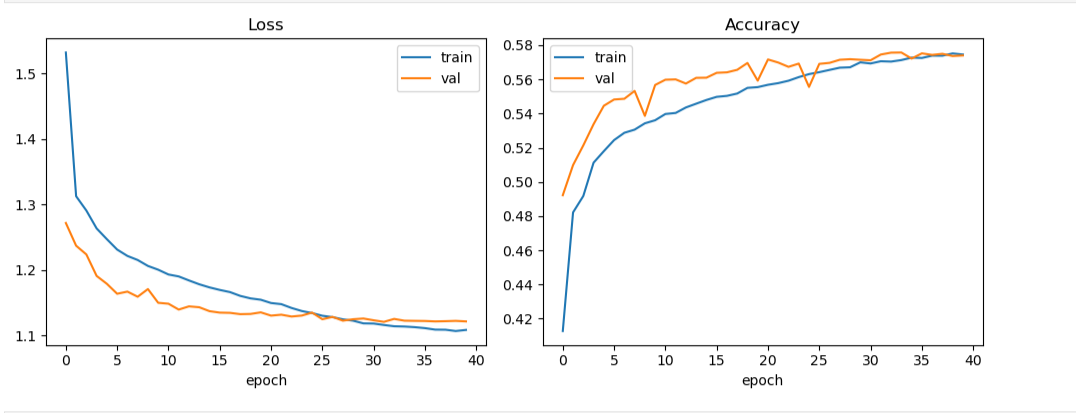
\includegraphics[width=0.9\textwidth]{fig_loss_accuracy.png}
    \caption{Training and validation loss/accuracy curves.}
    \label{fig:loss-accuracy}
\end{figure}

\section{Overall Classification Performance}
The overall test accuracy is approximately 0.574. The row-normalized confusion matrix in Figure~\ref{fig:cm-overall} shows strong performance on several digital modulations while revealing confusions among closely related classes.

\begin{figure}[H]
    \centering
    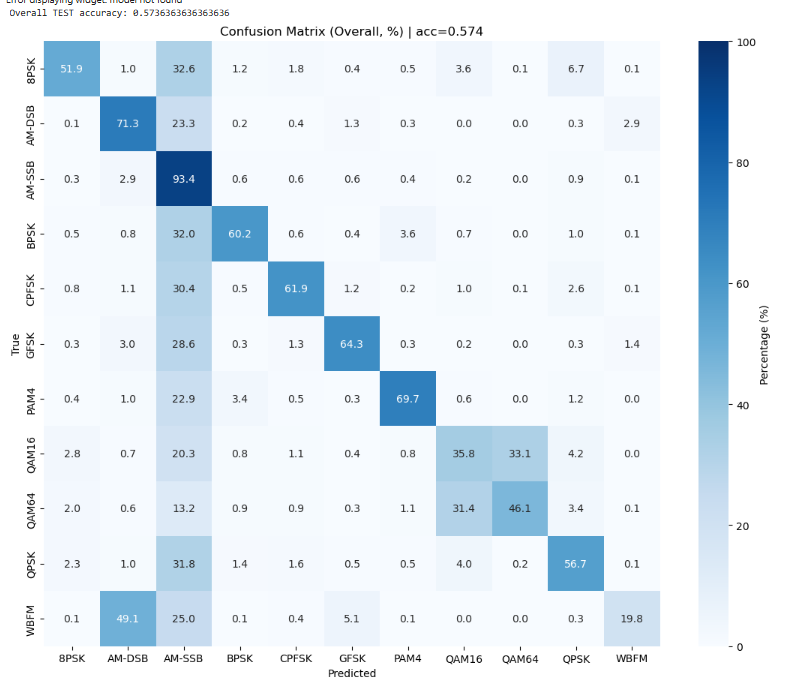
\includegraphics[width=0.85\textwidth]{fig_confusion_overall_percent.png}
    \caption{Overall confusion matrix (percentage, row-normalized).}
    \label{fig:cm-overall}
\end{figure}

\section{SNR-wise Performance}
Figure~\ref{fig:snr-acc} shows that accuracy increases with SNR, confirming the sensitivity of AMC performance to channel conditions.

\begin{figure}[H]
    \centering
    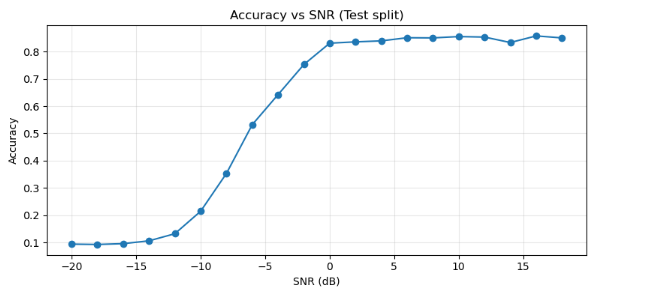
\includegraphics[width=0.8\textwidth]{fig_accuracy_vs_snr.png}
    \caption{Accuracy vs. SNR on the test split.}
    \label{fig:snr-acc}
\end{figure}

\section{High-SNR Confusion Analysis}
At 18 dB SNR, the confusion matrix (Figure~\ref{fig:cm-18db}) indicates clearer separation between classes, though similar modulation families still show occasional misclassification.

\begin{figure}[H]
    \centering
    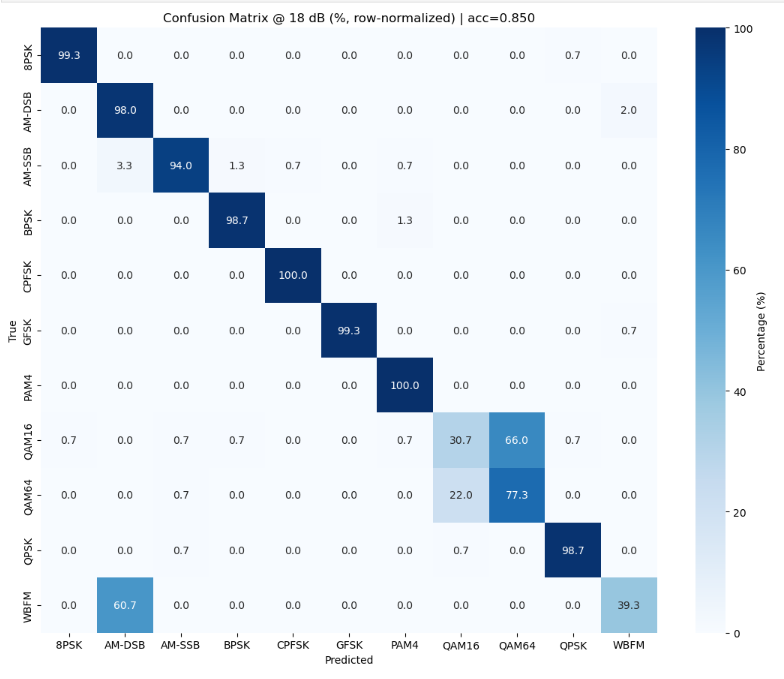
\includegraphics[width=0.8\textwidth]{fig_confusion_18db_percent.png}
    \caption{Confusion matrix at 18 dB SNR (percentage, row-normalized).}
    \label{fig:cm-18db}
\end{figure}

\section{Error Analysis and Observations}
Misclassifications are most common among QAM16 and QAM64 due to their closely related constellations, as well as between analog AM variants under low-SNR conditions. FSK-based modulations show improved accuracy at moderate SNR levels because their spectral signatures are more separable. The results emphasize the need for robust feature extraction and potentially longer context windows or recurrent layers for improved temporal modeling.

\section{Comparison to Prior Work}
The qualitative trends align with previous studies that report CNNs outperforming handcrafted features but remaining sensitive to low-SNR regimes~\cite{oshea2016cnn,oshea2018ota}. While deeper architectures can improve accuracy, they introduce additional computational complexity. The baseline presented here provides a reproducible reference for future work on architecture improvements, data augmentation, and domain adaptation.

\section{Practical Considerations}
For deployment in spectrum monitoring or cognitive radio systems, runtime constraints and robustness to unseen channel conditions are critical. Techniques such as transfer learning, model compression, and continual learning can help adapt AMC models to changing environments. The dataset-centric approach should be complemented with over-the-air validation to measure real-world performance.

\chapter{Conclusion and Future Work}
This project implemented a baseline CNN for automatic modulation classification on the RadioML 2016 dataset. The model achieved an overall test accuracy of about 0.574 and demonstrated clear SNR-dependent performance trends. The study highlights that compact CNNs provide a strong baseline while still leaving room for significant improvements in robustness and generalization.

\textbf{Contributions:}
\begin{itemize}
    \item Implemented a reproducible preprocessing and stratified data-splitting pipeline for RadioML 2016.10a.
    \item Designed and trained a compact 1D CNN for modulation recognition on raw I/Q sequences.
    \item Evaluated performance with overall accuracy, confusion matrices, and SNR-wise analysis.
    \item Documented theory, dataset characteristics, and practical considerations for AMC research.
\end{itemize}

\textbf{Limitations:} The model is evaluated on a fixed dataset and does not address real-time constraints or domain shift to other receivers and channels. The study does not explore data augmentation or model ensembles.

\textbf{Future Work:} Future efforts can explore deeper architectures, attention mechanisms, domain adaptation, data augmentation, and over-the-air validation. Incorporating signal impairments such as frequency offset and multipath in training can further improve robustness.

\appendix
\chapter{Modulation Class Descriptions}
\section{Summary of Modulation Characteristics}
Table~\ref{tab:class-desc} provides a brief description of each modulation class used in the dataset.

\begin{table}[H]
    \centering
    \caption{Modulation class descriptions.}
    \label{tab:class-desc}
    \begin{tabular}{p{0.28\textwidth} p{0.62\textwidth}}
        \toprule
        \textbf{Class} & \textbf{Description} \\
        \midrule
        8PSK & Eight-phase constellation with constant amplitude. \\
        BPSK & Two-phase constellation, robust but low spectral efficiency. \\
        QPSK & Four-phase constellation, widely used in digital systems. \\
        QAM16/QAM64 & Quadrature amplitude modulation with higher spectral efficiency. \\
        PAM4 & Four-level amplitude modulation, often used in baseband signaling. \\
        CPFSK & Continuous-phase FSK with smoother transitions. \\
        GFSK & FSK with Gaussian pulse shaping. \\
        AM-DSB & Double-sideband amplitude modulation. \\
        AM-SSB & Single-sideband amplitude modulation, improved bandwidth efficiency. \\
        WBFM & Wideband frequency modulation with high fidelity. \\
        \bottomrule
    \end{tabular}
\end{table}

\chapter{Project Workflow Summary}
The project workflow consists of dataset preparation, preprocessing, model design, training, evaluation, and result interpretation. Each stage is designed to be reproducible and modular, allowing future iterations to extend the baseline with additional data, architectures, and evaluation protocols.

\begin{thebibliography}{99}
\bibitem{haykin2005cognitive}
S. Haykin, ``Cognitive radio: Brain-empowered wireless communications,'' \textit{IEEE Journal on Selected Areas in Communications}, 2005.

\bibitem{proakis2001digital}
J. G. Proakis, \textit{Digital Communications}, 4th ed., McGraw-Hill, 2001.

\bibitem{sklar2001digital}
B. Sklar, \textit{Digital Communications: Fundamentals and Applications}, 2nd ed., Prentice Hall, 2001.

\bibitem{azzouznandi1996}
E. E. Azzouz and A. K. Nandi, \textit{Automatic Modulation Recognition of Communication Signals}, Springer, 1996.

\bibitem{gardner1988}
W. A. Gardner, ``Signal interception: A unifying theoretical framework for feature detection,'' \textit{IEEE Transactions on Communications}, 1988.

\bibitem{oshea2016dataset}
T. J. O’Shea and N. West, ``Radio Machine Learning Dataset Generation with GNU Radio,'' 2016.

\bibitem{oshea2016cnn}
T. J. O’Shea, J. Corgan, and T. C. Clancy, ``Convolutional Radio Modulation Recognition Networks,'' in \textit{International Conference on Engineering Applications of Neural Networks}, 2016.

\bibitem{oshea2018ota}
T. J. O’Shea, T. Roy, and T. C. Clancy, ``Over-the-Air Deep Learning Based Radio Signal Classification,'' \textit{IEEE Journal of Selected Topics in Signal Processing}, 2018.

\bibitem{rajendran2018dl}
S. Rajendran \textit{et al.}, ``Deep Learning Models for Wireless Signal Classification with Distributed Low-Cost Spectrum Sensors,'' \textit{IEEE Transactions on Cognitive Communications and Networking}, 2018.

\bibitem{lecun1998}
Y. LeCun, L. Bottou, Y. Bengio, and P. Haffner, ``Gradient-based learning applied to document recognition,'' \textit{Proceedings of the IEEE}, 1998.

\bibitem{goodfellow2016dl}
I. Goodfellow, Y. Bengio, and A. Courville, \textit{Deep Learning}, MIT Press, 2016.

\bibitem{loshchilov2019adamw}
I. Loshchilov and F. Hutter, ``Decoupled Weight Decay Regularization,'' in \textit{International Conference on Learning Representations}, 2019.

\bibitem{powers2011}
D. M. W. Powers, ``Evaluation: From Precision, Recall and F-measure to ROC, Informedness, Markedness and Correlation,'' \textit{Journal of Machine Learning Technologies}, 2011.

\bibitem{pytorchdocs}
PyTorch, ``PyTorch Documentation,'' [Online]. Available: \url{https://pytorch.org/docs/}
\end{thebibliography}

\end{document}
